\documentclass[11pt]{article}

\usepackage[margin=1in]{geometry}
\usepackage{amsmath, amssymb, amsthm}
\usepackage{graphicx}
\usepackage{hyperref}

\title{A Revised Theory Note for the On-Chain Gaussian Random Number Generator}
\author{Simon Tian}
\date{}

\newtheorem{theorem}{Theorem}
\newtheorem{remark}{Remark}

\begin{document}

\maketitle

\section{Introduction}

This note revises the probabilistic theory behind the on-chain Gaussian random
number generator built from the binary digits of a \texttt{keccak256} hashed
value. The main purpose is to state the assumptions more carefully and to align
the practical approximation with the theorem that is actually being used.

Let a hashed value produce a binary vector of length $n$, and let
$X_{n,1}, \dots, X_{n,n}$ denote the corresponding digits, where
$X_{n,i} = 1$ if the $i$-th digit is $1$ and $X_{n,i} = 0$ otherwise. The
quantity of interest is the count of $1$'s,
\[
S_n = \sum_{i=1}^n X_{n,i}.
\]

The classical iid Bernoulli model is stronger than what is needed here. In
practice, the bit probabilities need not be exactly equal to $0.5$. The more
appropriate model is to treat the digits as independent Bernoulli random
variables with bit-specific success probabilities
\[
\mathbb{P}(X_{n,i} = 1) = p_{n,i},
\]
where the values $p_{n,i}$ may vary with $i$ and may only be approximately
equal to $0.5$.

Under this model, the count $S_n$ has a Poisson-binomial distribution. The
theoretical justification for a Gaussian approximation is therefore not the iid
binomial model, but a central limit theorem for sums of independent,
non-identically distributed Bernoulli random variables.

\section{Empirical Motivation}

The accompanying numerical study does not prove the assumptions below, but it
does provide empirical support for them over several tested families of inputs.
The role of that study is to support the following working assumptions:

\begin{enumerate}
\item each bit has a success probability $p_{n,i}$ that is close to $0.5$;
\item there is no material empirical evidence of cross-bit dependence within a
hashed output for the tested input families;
\item there is no material empirical evidence of serial dependence across the
tested sequential inputs.
\end{enumerate}

These points justify modeling the digits as independent Bernoulli variables with
possibly different success probabilities. The empirical study should therefore
be viewed as support for the modeling assumptions, rather than as a formal proof
of them. In particular, the study speaks to selected finite-sample diagnostics
over tested input families; it does not establish full joint independence of the
\texttt{keccak256} output bits as a theorem.

\section{Probabilistic Model}

For each $n$, assume that
\[
X_{n,1}, \dots, X_{n,n}
\]
are independent Bernoulli random variables with
\[
\mathbb{P}(X_{n,i}=1)=p_{n,i}, \qquad
\mathbb{E}[X_{n,i}] = p_{n,i}, \qquad
\mathrm{Var}(X_{n,i}) = p_{n,i}(1-p_{n,i}).
\]

Define the mean and variance of the count by
\[
\mu_n = \sum_{i=1}^n p_{n,i},
\qquad
\sigma_n^2 = \sum_{i=1}^n p_{n,i}(1-p_{n,i}).
\]

Then the natural standardized count is
\[
Z_n = \frac{S_n - \mu_n}{\sigma_n}.
\]

This formulation is more general than the iid Bernoulli$(0.5)$ model and fits
the intended application better.

\section{Lyapunov Central Limit Theorem}

\begin{theorem}
Suppose that for each $n$ the family
\[
X_{n,1}, \dots, X_{n,n}
\]
consists of independent Bernoulli random variables with success probabilities
$p_{n,1}, \dots, p_{n,n}$. Assume there exists a constant
$\varepsilon \in (0, 1/2)$ such that
\[
\varepsilon \le p_{n,i} \le 1-\varepsilon
\]
for all relevant $n$ and $i$. Then Lyapunov's condition holds for $\delta = 1$,
and
\[
\frac{S_n - \mu_n}{\sigma_n}
\xrightarrow{d}
\mathcal{N}(0,1)
\qquad \text{as } n \to \infty.
\]
\end{theorem}

\begin{proof}
For Bernoulli random variables,
\[
\mathbb{E}\left[\left|X_{n,i} - p_{n,i}\right|^3\right]
= p_{n,i}(1-p_{n,i})^3 + (1-p_{n,i})p_{n,i}^3.
\]
The right-hand side is maximized at $p_{n,i}=1/2$, so
\[
\mathbb{E}\left[\left|X_{n,i} - p_{n,i}\right|^3\right] \le \frac{1}{8}.
\]
Hence
\[
\sum_{i=1}^n \mathbb{E}\left[\left|X_{n,i} - p_{n,i}\right|^3\right]
= O(n).
\]

On the other hand, the lower bound on $p_{n,i}$ implies
\[
p_{n,i}(1-p_{n,i}) \ge \varepsilon(1-\varepsilon),
\]
and therefore
\[
\sigma_n^2
= \sum_{i=1}^n p_{n,i}(1-p_{n,i})
\ge n \varepsilon(1-\varepsilon).
\]
It follows that
\[
\sigma_n^3 \ge \left(n \varepsilon(1-\varepsilon)\right)^{3/2}.
\]
Thus the Lyapunov ratio for $\delta = 1$ satisfies
\[
\frac{1}{\sigma_n^3}
\sum_{i=1}^n \mathbb{E}\left[\left|X_{n,i} - p_{n,i}\right|^3\right]
= O(n^{-1/2}) \to 0.
\]
By Lyapunov's central limit theorem,
\[
\frac{S_n - \mu_n}{\sigma_n}
\xrightarrow{d}
\mathcal{N}(0,1).
\]
\end{proof}

\section{Interpretation for \texttt{keccak256}}

For a \texttt{keccak256} hashed value, the natural choice is $n=256$. The
theorem above gives an asymptotic justification for the Gaussian approximation
to the standardized count of $1$'s. In practice, the numerical study suggests
that the probabilities $p_i$ are close to $0.5$, so the mean and variance are
close to
\[
\mu = \sum_{i=1}^{256} p_i \approx 128,
\qquad
\sigma^2 = \sum_{i=1}^{256} p_i(1-p_i) \approx 64.
\]
This yields the practical approximation
\[
\frac{S - 128}{8} \approx \mathcal{N}(0,1).
\]

\begin{figure}[htbp]
\centering
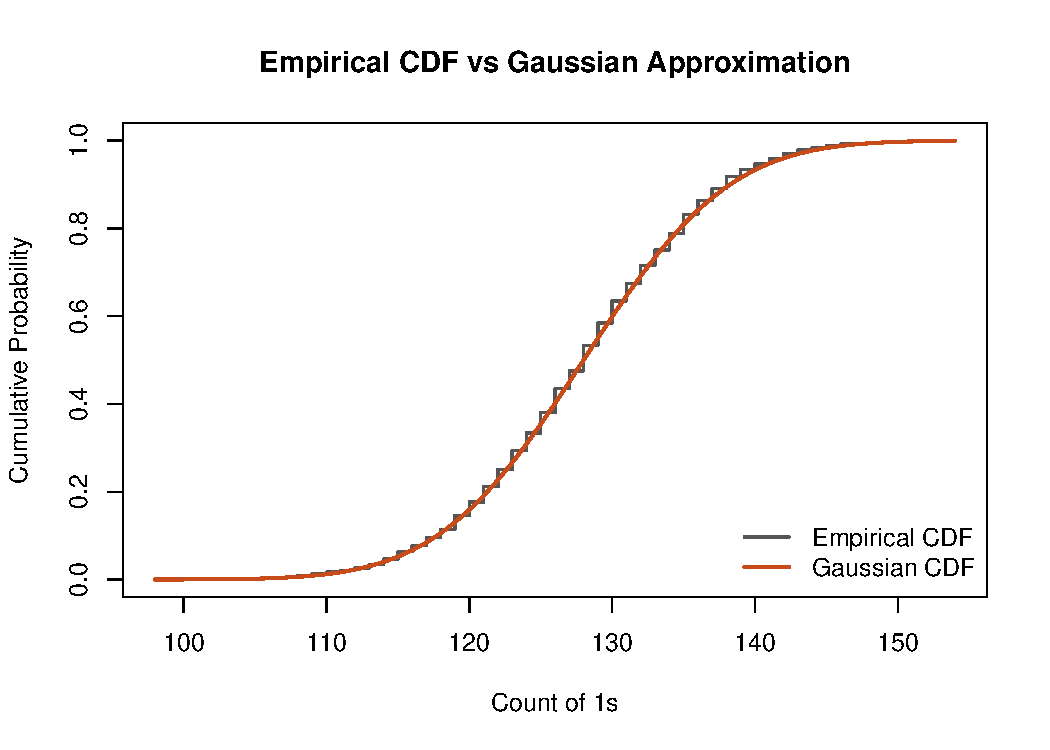
\includegraphics[width=0.8\textwidth]{NumericalStudy/figures/popcount_cdf.pdf}
\caption{Empirical CDF of $3{,}000$ simulated counts of $1$'s against the
Gaussian CDF with mean $128$ and standard deviation $8$.}
\label{fig:popcount-cdf}
\end{figure}

To make the approximation error more explicit, write
\[
p_i = \frac{1}{2} + e_i.
\]
Then
\[
\mu = \sum_{i=1}^{256} p_i = 128 + \sum_{i=1}^{256} e_i,
\]
and
\[
\sigma^2
= \sum_{i=1}^{256} p_i(1-p_i)
= \sum_{i=1}^{256} \left(\frac{1}{4} - e_i^2\right)
= 64 - \sum_{i=1}^{256} e_i^2.
\]
Therefore the variance error is second-order in the bit biases. If the
empirical deviations $e_i$ are small, then the practical normalization
$(S-128)/8$ is close to the theoretically natural normalization
$(S-\mu)/\sigma$.

\section{Scaled Solidity Output}

Solidity does not support floating-point arithmetic natively, so the
standardized variable can be scaled by a factor of $1000$. If
\[
Y = \frac{S-128}{8},
\]
then define
\[
Z = 1000Y = 125S - 16000.
\]
This is the integer-valued approximation used to represent the Gaussian random
number on-chain with three decimal digits of precision.

\section{Scope and Limitations}

\begin{remark}
The numerical study provides empirical support for the independence assumption,
but it does not prove full joint independence of all $256$ digits.
\end{remark}

\begin{remark}
Lyapunov's theorem justifies the Gaussian approximation under independence and
non-degeneracy of the success probabilities. It does not justify the
approximation if there is genuine dependence among the bits.
\end{remark}

\begin{remark}
The theorem is asymptotic, whereas the intended application uses the fixed value
$n=256$. The practical approximation is therefore supported by both the CLT
heuristic and the empirical evidence that the bit probabilities are close to
$0.5$.
\end{remark}

\section{Conclusion}

The clean theoretical statement is as follows: model the digits of a
\texttt{keccak256} hashed value as independent Bernoulli random variables with
possibly different success probabilities $p_i$. Under this model, the count of
$1$'s has a Poisson-binomial distribution, and Lyapunov's central limit theorem
implies that the standardized count is asymptotically Gaussian. The empirical
study then motivates the practical approximation
\[
\frac{S-128}{8} \approx \mathcal{N}(0,1),
\]
which leads directly to the scaled on-chain representation
\[
125S - 16000.
\]

\end{document}
